To verify the correctness of the manual calculations, the circuit was recreated on the online platform \textbf{Quirk} (\url{https://algassert.com/quirk}).
The offline copy of the circuit can be seen at \cref{fig:quirk1}.
\begin{figure}[H]
\centering
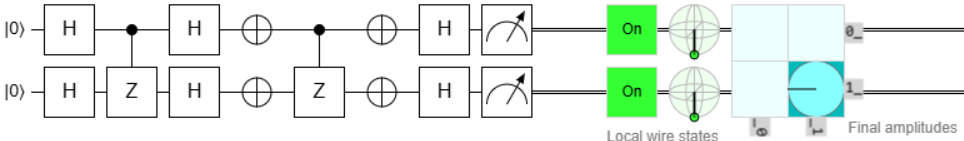
\includegraphics[width=0.9\linewidth]{circuits/Quirk_1.png}
\caption{Circuit quirk ex02.}
\label{fig:quirk1}
\end{figure}

From the \textit{State Vector Display} in Quirk, it can be observed that the final state of the system matches with the manually calculated result.
